\documentclass[10pt,sans,english,compress,xcolor=dvipsnames]{beamer}
\author[Lily ]{ Dr Lily Asquith (Lily, she/her)}

\usetheme{Szeged}
%\defbeamertemplateparent{enumerate items}{enumerate item,enumerate subitem,enumerate subsubitem,enumerate mini template}
\definecolor{titcol}{RGB}{16,78,100} 
\setbeamercolor{frametitle}{fg=titcol,bg=White}
\useoutertheme{miniframes} 
\useinnertheme{rectangles}

\usepackage{pifont}
\newcommand{\tick}{\textcolor{grn}{\ding{52} } }
\newcommand{\nope}{\textcolor{red}{\ding{54} } }


\usepackage{soul}
\usepackage{cancel}

\usepackage[most]{tcolorbox}
\definecolor{LilyBlack}{rgb}{0.05,0.1,0.3} % UBC Blue (primary)
\usecolortheme[named=LilyBlack]{structure}

\usepackage{booktabs}
\usepackage{tabularx}
%\usepackage{tikz}
%\def\checkmark{\tikz\fill[scale=0.4](0,.35) -- (.25,0) -- (1,.7) -- (.25,.15) -- cycle;}

\usepackage{physics}

\usepackage{xparse}

\setbeamertemplate{footline}{%
  \leavevmode%
  \hbox{\begin{beamercolorbox}[wd=.5\paperwidth,ht=2.5ex,dp=1.125ex,leftskip=.3cm plus1fill,rightskip=.3cm]{author in head/foot}%
    \usebeamerfont{author in head/foot}\insertshortauthor
  \end{beamercolorbox}%
  \begin{beamercolorbox}[wd=.5\paperwidth,ht=2.5ex,dp=1.125ex,leftskip=.3cm,rightskip=.3cm plus1fil]{title in head/foot}%
    \usebeamerfont{title in head/foot}\insertshorttitle\hfill\insertframenumber\,/\,\inserttotalframenumber
  \end{beamercolorbox}}%
  \vskip0pt%
}

\DeclareMathSizes{10}{10}{6}{4} % this one
%\DeclareMathSizes{10.95}{10}{6}{4}   % For size 10 text

\newcommand*\ColorBox[3][black]{%
  \makebox[2em][c]{%
    \setlength\fboxsep{-.5\fboxrule}%
    \raisebox{\dimexpr-#3em+.5ex}{%
      \fcolorbox{#1}{#2}{%
        \rule{0pt}{\dimexpr#3em*2}%
        \rule{\dimexpr#3em*2}{0pt}%
      }%
    }%
  }%
}

\usepackage{hyperref}
\hypersetup{
    colorlinks=true,
    linkcolor=blue,
    filecolor=magenta,      
    urlcolor=blue,
    pdftitle={Overleaf Example},
    pdfpagemode=FullScreen,
    }

\urlstyle{same}

% this part excludes specified frames from counters in navigation bar
\makeatletter
\let\beamer@writeslidentry@miniframeson=\beamer@writeslidentry
\def\beamer@writeslidentry@miniframesoff{%
  \expandafter\beamer@ifempty\expandafter{\beamer@framestartpage}{}% does not happen normally
  {%else
    % removed \addtocontents commands
    \clearpage\beamer@notesactions%
  }
}
\newcommand*{\miniframeson}{\let\beamer@writeslidentry=\beamer@writeslidentry@miniframeson}
\newcommand*{\miniframesoff}{\let\beamer@writeslidentry=\beamer@writeslidentry@miniframesoff}
\makeatother


\makeatletter
\newcommand\notsotiny{\@setfontsize\notsotiny{6.5}{7.5}}
\makeatother




\usepackage{multicol}
\usepackage{sansmath}
\usepackage{minted}
\definecolor{LightGray}{gray}{0.95}
\usepackage{nicematrix}
%\usepackage{statmath}
\usepackage{pifont}
\newcommand{\tick}{\textcolor{grn}{\ding{52} } }
\newcommand{\nope}{\textcolor{red}{\ding{54} } }

\title[Tools]{Tools: Random Numbers, Monte Carlo, Intro to Estimators}
\date{}
\titlegraphic{
%\center

\includegraphics[scale=0.15]{sussex-logo}
}
% Lily includes for font and spacing
\usepackage{cmbright} % pretty nice but maybe a bit too different
\renewcommand{\baselinestretch}{1.1} 
\usepackage{sansmath}
% Lily highlight numerical answers for quicker marking
\usepackage{xcolor}
\definecolor{mygreen}{RGB}{226,254,226}
\definecolor{mylblue}{RGB}{205, 248, 250}
\definecolor{mylpink}{RGB}{159, 43, 104}
\usepackage[most]{tcolorbox}

\newtcbox[auto counter]{\ghl}
{enhanced, on line, boxsep=0pt,left=6pt,right=6pt,top=2pt,bottom=2pt,rightrule=1pt,
colback=mygreen,
colframe=black 
}
\newtcbox[auto counter]{\bhl}
{enhanced, on line, boxsep=0pt,left=6pt,right=6pt,top=2pt,bottom=2pt,rightrule=1pt,
colback=mylblue,
colframe=black 
}
\newtcbox[auto counter]{\yhl}
{enhanced, on line, boxsep=0pt,left=2pt,right=2pt,top=1pt,bottom=1pt,rightrule=1pt,
colback=lyellow,
colframe=black 
}

\newcommand{\bhlm}[1]{\bhl{$#1$}}

\newtcbox[auto counter]{\phl}
{enhanced, on line, boxsep=0pt,left=6pt,right=6pt,top=2pt,bottom=2pt,rightrule=1pt,
colback=mylpink,
colframe=black 
}

\DeclareMathOperator*{\plim}{plim}
\begin{document}

\newcommand\info{\mathcal{J}_{\theta}}
\newcommand\loglike{\ln{ \mathcal{L}_{\theta}} }
\newcommand\like{\mathcal{L}_{\theta} }

\newcommand\thetahat{\hat{ \theta }  }

\definecolor{grn}{RGB}{0,128,0} 
\newcommand{\gbl}[1]{\textcolor{grn}{#1}}

\definecolor{wh}{rgb}{0.95, 0.95, 0.96}
\newcommand{\wht}[1]{\textcolor{wh}{#1}}

%\newcommand{\inprob}{\overset{p}{\to}}

\newcommand{\boo}[1]{\textbf{\textcolor{red}{#1}}}

\newcommand{\covmat}{\mathbf{\textcolor{magenta}{\Sigma}} }


\definecolor{purr}{RGB}{128,0,128} 
\newcommand{\purp}[1]{\textcolor{purr}{#1}}

\newcommand{\magt}[1]{\textbf{\textcolor{magenta}{#1}}}
 \newcommand{\magtn}[1]{\textcolor{magenta}{#1}}
 
%\definecolor{bbl}{RGB}{128,0,128} 
\newcommand{\bbl}[1]{\textcolor{blue}{#1}}

\newcommand{\rbl}[1]{\textcolor{red}{#1}}

\definecolor{dblu}{RGB}{37,150,190} 
\newcommand{\blu}[1]{\textcolor{dblu}{#1} }

\definecolor{dor}{RGB}{255,40,0} 
\newcommand{\dor}[1]{\textcolor{dor}{#1} }

\definecolor{darkgreen}{RGB}{46,139,87} 
\newcommand{\dgreen}[1]{\textbf{\textcolor{darkgreen}{#1}} }
%\newcommand{\gbl}[1]{\textcolor{darkgreen}{#1}}

\definecolor{lgray}{RGB}{222,222,222} 

\definecolor{lyellow}{RGB}{255,255,224} 

\newcommand{\E}[1]{\mathbf{E}_{#1}}
%
\newcommand{\rvX}[1]{X_{(#1)} } 

\newcommand{\rvY}[1]{Y_{(#1)} }

\newcommand{\rvx}[1]{x_{(#1)} } 

\newcommand{\rvy}[1]{y_{(#1)} }



\newcommand{\red}[1]{\textcolor{red}{#1} }

\newcommand{\bluedots}{\blu{\ldots} }

\newcommand{\dordots}{\dor{\ldots} }


\newcommand{\where}{\dgreen{\;where\;} }


\newcommand{\pand}{\dgreen{\;and\;} }
\newcommand{\por}{\dgreen{\;or\;} }

\newcommand{\sumN}{ \sum\limits_{\blu{i}}^{\blu{N}} }

\newcommand{\sumZ}{ \sum\limits_{\dor{j}}^{\dor{Z}} }

\newcommand{\Expec}[1]{ \mathbb{E}[#1] }


\newcommand{\Xfj}[1]{ X_{ \dor{#1} } }

\newcommand{\xfi}[1]{ x_{ \blu{#1} } }

\newcommand{\Xij}[2]{ X_{\mage{#1},\blu{#2} }}

\newcommand{\sumxi}{ \sumN \xfi{i} }

\newcommand{\sumXj}{ \sumZ \Xfj{j} }

\newcommand{\sumZa}[1]{ \sumZ {#1}_{ \dor{j} } }

\newcommand{\sumZab}[2]{ \sumZ {#1}_{ \dor{j} }\, {#2}_{ \dor{j} } }

\newcommand{\sumNab}[2]{ \sumN {#1}_{ \blu{i} }\, {#2}_{ \blu{i} } }

\newcommand{\vecxi }{ [ \xfi{1} \xfi{2}, \bluedots, \xfi{N} ] }

\newcommand{\vecXj }{ [ \Xfj{1} \Xfj{2}, \bluedots, \Xfj{Z} ] }

\newcommand{\vecXij }{ [ \Xij{1}{1} \Xij{1}{2}, \bluedots, \Xij{1}{N_1} ],\, [ \Xij{2}{1} \Xij{2}{2}, \bluedots, \Xij{2}{N_2} ],\, \dordots,\,[ \Xij{Z}{1} \Xij{Z}{2}, \bluedots, \Xij{Z}{N_Z} ] }

% definitions

\newcommand{\overNblack}{ \dfrac{1}{N} }
\newcommand{\overN}{ \dfrac{1}{ \blu{N} } }

\newcommand{\defmean }{ \overline{x} = \overN \sumN \xfi{i} }

\newcommand{\meanx }{ \overline{x} }
\newcommand{\meansqx }{ \overline{x^2} }
\newcommand{\sqmeanx }{ \overline{x}^2 }
\newcommand{\devsq}{ (\xfi{i} - \meanx)^2 }

%\newcommand{\var }[1]{ \mathcal{V}_{#1} }
\newcommand{\defvar }{ \var{x} = \overN \sumN \devsq }
\newcommand{\defvarshort }{ \var{x} = \meansqx - \sqmeanx }

\newcommand{\defstd }{ s_x = \sqrt{ \var{x} }  }

\newcommand{\defwmean }{ \overline{X} = \dfrac{ \sumZab{w}{X} }{ \sumZa{w} } }  

\newcommand{\defw }{ w_{\dor{j}} = \dfrac{1}{ \var{\Xfj{j} } } }



\begin{frame}
\titlepage
\end{frame} 

%\section*{Preamble}




% contents
\begin{frame}{Tools}
\begin{itemize}
\item Random/Pseudorandom Numbers
\item Monte Carlo
\item Requirements for an Estimator
\item Sample Mean and Variance as Estimators
\item Likelihood and Bayes recap
\item Maximum Likelihood, Least Squares, Residuals, Chi Squared
\end{itemize}

\end{frame} 


\begin{frame}{Intro, reminder of big picture}

\footnotesize

Estimating parameters and their uncertainties has been our goal, and we are now pretty much ready to do that.\\[1ex]
We have used \magt{PseudoRandom Number Generators} many times already, every time we pull a set of RVs from a scipy.stats pdf for example. We will give a little nod to where they come from.\\[1ex]
\magt{Monte Carlo} methods are important for simulating fake data and for estimating parameters.\\[1ex]
We will see that \magt{Parameter Estimation} comes down to maximising the Likelihood function, or equivalently to minimising the residuals (Chi Squared is the sum of the squared residuals).\\[1ex]
Next week we will go through Maximum Likelihood Estimation in full. The process is much more intuitive and friendly than some descriptions would have us believe. There are a few bits of math, but we will be grand I think.

\end{frame} 



% RANDOM NUMBERS


\section{Random Numbers}

\begin{frame}{Random Numbers}
\footnotesize
\centering

\includegraphics[scale=0.38]{dilbert2.jpg}
\tiny

Credit: DILBERT © 2001 Scott Adams [All rights reserved].
\end{frame} 



\begin{frame}{Random Numbers}
\footnotesize
A Random Number  is a term used to describe a value that is produced by a random (unpredictable) process.\\[1ex]

 There are many things in the physical world that exhibit random behaviour (such as quantum mechanical processes), but the instruments we use to measure the behaviour often destroy/hide the randomness. \\[1ex]
 
 We can extract (a limited number of) truly random numbers from eg \href{https://www.random.org/}{random.org}, which uses atmospheric noise.\\[1ex]
 
True Random Number Generation (TRNG) is an active area of research, and is  rapidly changing. Whatever I write here will probably be out of date in two years. A recent exciting development was \href{https://www.nature.com/articles/s41586-025-09054-3}{published in Nature} this summer.

\end{frame} 


\begin{frame}[fragile]{PseudoRandom Numbers (PRNs)}
\footnotesize
A Pseudorandom Number is a term used to describe a number in a sequence that appears random, but is produced by a deterministic\magt{*} process. \\[1ex]

Note that when we draw RVs from a distribution using python libraries, we are using their PseudoRandom Number Generators (PRNGs).
\begin{minted}[bgcolor=LightGray]{python}
from numpy import random
# It is called random, but should be called pseudorandom
crvs_x = random.uniform(0,100,10)  
\end{minted}

Human beings tend to have fixed ideas of what random should look like, which is amusing if you think about it. If you truly had a random shuffle on your music playlist, you would get many repetitions. People don't like that.

\magtn{*Deterministic: an outcome is caused by preceding events.}
\end{frame} 


\begin{frame}[fragile]{An Outdated PRNG}
\footnotesize
A Multiplicative Linear Congruential\magtn{*} Generator (MLCG)  is an algorithm that produces sequences of pseudorandom numbers using the rule:
\begin{center}
 $n_{i+1} = a\, n_i\, mod(m)$\\[1ex]
 \end{center}
The parameters $a$, $m$ and $n_0$ ($n_0$ is the \boo{Seed}) must be chosen with care to ensure the periodicity does not cause problems. Check out the terrible example of choices below where the produced sequence repeats after just 6 numbers.
 \notsotiny
\begin{minted}[bgcolor=LightGray]{python}
# DEMO of MLCG PERIODICITY - repeats after six numbers!#
import numpy as np
def MLCG(a, m, seed, size):
    sequence = np.zeros(size)
    sequence[0] = seed
    for i in range(0, size-1):
        sequence[i+1] = (a * sequence[i]) % m
    return sequence
print( MLCG(a=3, m=7, seed=1, size=10) ) #[1. 3. 2. 6. 4. 5. 1. 3. 2. 6.]
\end{minted}
 \vspace{0.2cm}
 \footnotesize
\magtn{Congruence: the quality or state of agreeing, coinciding.}\\
  
\end{frame} 


\begin{frame}[fragile]{Linear Congruential Generators}
\footnotesize
A modification to improve the MLCG behaviour is to use an increment $c$ such that the Linear Congruential Generator (LCG) is:
\begin{center}
 $n_{i+1} = (a\, n_i\, + c)\, mod(m)$
  \end{center}
 It is still crucial to choose the parameters with care. The C programming language used  $a=1,664,525$  based on a bunch of research into behaviour of numbers. \\[1ex]

The modulus $m$ should be a prime or power of 2 (for efficiency of computation) and should be large enough to ensure the minimum level of periodicity for whatever you are doing.\\[1ex]
 
\bbl{Note that the PRNs supplied by eg python libraries are state-of-the-art and it is very unlikely you will want to employ your own methods! }
\end{frame} 

\begin{frame}[fragile]{The Seed}
\footnotesize
\magtn{The Seed} is a starting value that entirely controls the sequence of pseudorandom numbers produced.\\[1ex]

If we use the same seed in a PRNG, we will get the same sequence. This is very useful for testing.\\[1ex]

With python  we have to set the seed to the same value \bbl{every time we call rand} (for example), otherwise the sequence will use a different seed (note that this is not thread-safe).\\[1ex]

If you do not set the seed, numpy/scipy will set it using nondeterministic data from your computer operating system.\\[1ex]
\end{frame} 



\begin{frame}[fragile]{The Seed}
\footnotesize
\begin{minted}[bgcolor=LightGray]{python}
# DEMO of SEED #
import numpy as np
from numpy import random
np.random.seed(0) # set the seed
np.random.rand(3) # generate 3 PRNs
#array([0.5488135 , 0.71518937, 0.60276338])
np.random.seed(0) # set the seed
np.random.rand(3) # generate 3 PRNs
#array([0.5488135 , 0.71518937, 0.60276338])
np.random.rand(3) # generate 3 PRNs without setting the seed
#array([0.54488318, 0.4236548 , 0.64589411])
\end{minted}

\magt{We cannot just set the seed once and then call the generator over and over again and expect the same sequence.}
\end{frame} 

\begin{frame}[fragile]{The Mersenne Twister \& PCG}
\footnotesize
The \boo{Mersenne Twister} is an algorithm used by python and most other programming languages to generate pseudorandom numbers. \\[1ex]

It is named for its use of the Mersenne prime,  $2^{19937} -1$, as the period length. It is called a Twister because it's a cool name and because it is a `twisted' version of an earlier algorithm (GFSR).\\[1ex]

\boo{PCG64}  (Permuted Congruential Generator, 64-bit) is the PRNG used by numpy. I tested it, and it is faster than the scipy default Mersenne Twister!\\[1ex]

For those interested in the algorithms, see the \href{https://www.nature.com/articles/s41586-025-09054-3}{1997 Mersenne Twister paper} from Matsumoto \& Nishimura and the \href{https://www.pcg-random.org/pdf/hmc-cs-2014-0905.pdf}{2014 PCG paper} from O'Neill.

\end{frame} 

\begin{frame}[fragile]{PCG (numpy) versus Mersenne Twister (scipy)}
\footnotesize
Note: to do this test properly you would want to do it many times and take the average.\\
\notsotiny
\begin{minted}[bgcolor=LightGray]{python}
import timeit
N=1_000
glob = {'N': N}
t_sp = timeit.timeit(setup='import scipy as sp; 
sp_init = sp.stats.norm()', 
stmt='sp_init.rvs(size=N)',globals=glob )
print("Scipy MT time:{} for {} norm PRNS.".format(  t_sp, N ) )

t_np = timeit.timeit(setup='import numpy as np; 
np_init= np.random.default_rng()', 
stmt='np_init.normal(size=N)',globals=glob )
print("Numpy PCG64 time:{} for {} norm PRNS.".format( t_np, N) )

> Scipy MT time:27.727043333999998 for 1000 norm PRNS.
> Numpy PCG64 time:5.511924125000004 for 1000 norm PRNS.
\end{minted}
\end{frame} 




% MONTE CARLO


\section{Monte Carlo}

\begin{frame}{The Monte Carlo Method}
\footnotesize
%Monte Carlo Simulation is a technique for calculating probabilities using (pseudo)random sampling.\\ 
\magtn{Monte Carlo} is a code name, because during WW2 everything had to have a stupid name, because spies. \\[1ex]  

Stanislaw Ulam was playing solitaire, and wanted to know the probability of it coming out successfully. He wondered if the best way to determine this wouldn't be to just play the game a very large number of times and observe the frequency of success. \\[1ex]

Ulam's `brute force sampling' idea coincided (not a random coincidence) with the invention of computers, so it turned out to be a very good one. \\[1ex]

Ulam apparently stated that it would do okay `until the mathematicians arrive'. It seems like they have not yet arrived.\\
 
\end{frame} 


\begin{frame}{The Monte Carlo Method}
\footnotesize
 In its simplest form, the Monte Carlo method involves `rolling a dice' (aka using a PRNG) to create random data points that can be used for estimating something.\\[1ex]
 
 In its more general form, the Monte Carlo Method involves a bit more than just dice rolling. Sequences of PRNs can be generated using an algorithm such as the Mersenne Twister, and then may need to undergo some \magtn{Transformation} such that they produce whatever distribution is of interest to the user. The values extracted from the transform can be used to estimate some property of the `fake data' produced.\\[1ex]
 
\bbl{Python methods produce PRNs drawn from a large choice of distributions, so the Transform part of the MC Method is less relevant than it was back in the day when we could only produce basic (uniform) PRN sequences.}
 
 \end{frame} 

\begin{frame}{Transformation of PRN Sequences}
\footnotesize
The \magtn{Transformation Method} converts a uniform (flat) distribution of random numbers $U$  into a shapely distribution of choice $X$ by determining the function  $X(U)$. This is done by integrating the PDF and setting it to $U$, then solving for $X$.\\[1ex]

The \magtn{Acceptance/Rejection Method}  is a `hit and miss', method that can be used when the integral is too tricky. It involves drawing a box to contain our distribution, and then creating a histogram (more boxes) to define acceptable areas for our uniform numbers to fall in. This method can be very inefficient, but can be improved by drawing something a little more complicated than a single box (like , two boxes...)\\[1ex]

The \magtn{Weighted Sampling Method} uses all of the uniform PRNs, and stores a weight corresponding to the value of the (desired) PDF at that point. Then, whenever the PRN is used (to fill histograms etc), we can weight the event accordingly. \\[1ex]

\end{frame} 

\begin{frame}{Example: Transformation Method}
\footnotesize
Uniformly distributed sequence: $u = \{u_1, u_2, ..., u_n\}$\\[1ex]

We want them to be $x\sim Expon(\lambda)$:  $f_X(x;\lambda) = \lambda e^{-\lambda x}$\\[1ex]

$u = \int\limits_0^{x}  \lambda e^{-\lambda x} dx =   \bbl{-\dfrac{1}{\lambda}} \lambda e^{-\lambda x}\bigg|^{x}_0 =  -1 [ e^{-\lambda x}  -  e^{-\lambda 0} ] = 1 - e^{-\lambda x} $\\

$1 - u = e^{-\lambda x} $\\

$\ln{ (1 - u) }  = - \lambda x $\\

$- \dfrac{ 1 }{\lambda} \ln{ (1 - u) }  =  x(u) $ : we have an exponentially distributed sequence, $x$\\[1ex]

\magt{I am sure you can imagine, this is a very simple example of something that can be very complex!}
\end{frame} 


%
%
%\begin{frame}{Monte Carlo Integration}
%\footnotesize
% Monte Carlo Integration can be used to approximate the solutions to tricky integrals. The idea is that the integral of a function is just equal to its average (times the range over which the function is measured), and that the average itself can be found by random sampling. 
%
%\end{frame} 


% ESTIMATORS
\section{Estimators}

\begin{frame}{Point Estimators}
\footnotesize
A True Parameter (or set of parameters) is $\theta$. We estimate the value of this parameter using a dataset of measurements $x_{obs}$.\\[1ex]

A \magt{Point Estimator} is a function we use to make the Estimate: \magt{ $\hat{\theta}(x_{obs})$}\\[1ex]

The value returned by the function is the Point Estimate  $\hat{\theta}$ of the true parameter $\theta$.\\[1ex]

We use `hat notation' to indicate an Estimate (value, or Statistic) and to indicate an Estimator (function, or Statistic!):\\

\centering
\ghl{$\hat{\theta}$ = $\hat{\theta}(x_{obs})$}\\[2ex]

\end{frame} 

\begin{frame}{Side note on Statistics}
\footnotesize
\magtn{A Statistic is a property of the data}. Examples include:\\[1ex]

The \magtn{sample} mean: $\dfrac{1}{N} \sum\limits_i^N x_i $ (also the mode, median)\\[1ex]

The \magtn{sample} variance: $\dfrac{1}{N} \sum\limits_i^N (x_i-\overline{x})^2 $ (also the standard deviation).\\[1ex]

The minimum value of a \magtn{dataset}: $\min(x)$ (also the maximum, also any function of these).\\[1ex]

The most likely value of a parameter, \magtn{given the data}: $\hat{\theta} = argmax(\ln{\mathcal{L}_{\theta}})$.\\[1ex]

\bbl{The Expected Value $\mu=E[X]$ and True Variance $V[X]$ are not statistics, as they do not rely on the data.}

\end{frame} 


\begin{frame}{Interval Estimator}
\footnotesize
An \magtn{Interval Estimator} for a parameter is also a function $\hat{\theta}(x_{obs})$ computed on a dataset $x_{obs}$. \\

Rather than returning a single value (as per a point estimator), it returns:
\begin{enumerate}
\item A range (upper and lower boundary): the Confidence Interval \\
\item A Confidence Level\\[1ex]
\end{enumerate}
\vspace{0.5cm}

For example, an Interval Estimator might return a Confidence Interval of $(3.20, 3.25)$ and a Confidence Level of $99\%$\magt{*} \\

\magtn{* Recall the meaning of this is that in $99\%$ of repetitions of the experiment, we would expect to find a value between $(3.20, 3.25)$}\\

\end{frame} 


\begin{frame}{Requirements for an Estimator}
\footnotesize

An Estimator is constructed with the aim of being Consistent, Unbiased, and having Minimum Variance. In English: we want our Estimator to produce a good estimate.\\

\magtn{Consistent}: Estimate should approach true value as $N\to\infty$.\\

\hspace{2cm} \bhl{$\hat{\theta} \to \theta\; as \; N\to \infty$}\\[1ex]

\magtn{Unbiased}: The difference between estimate and the true parameter should be small, preferably zero.\\

\hspace{2cm} \bhl{$b = E[\hat{\theta}] - \theta $}\\[1ex]

\magtn{Minimum Variance}: We don't want too much spread in the estimated values (we want \textit{consistency}, but we used that word already).\\

\hspace{2cm} \bhl{$V[ \hat{\theta} ] = E[\hat{\theta}^2] - E^2[\hat{\theta}] \;\; \equiv \;\; E[ (\hat{\theta} - \mu)^2]$}\\[1ex]
\end{frame} 


\begin{frame}{Bias and Variance: Visually}
\footnotesize
\begin{center}
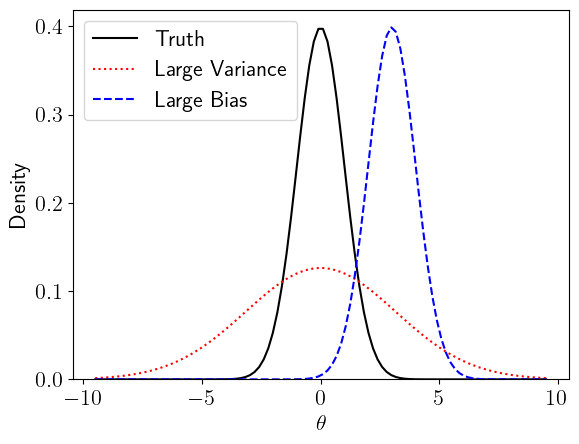
\includegraphics[scale=0.6]{Goldilocks.png}
\end{center}
\end{frame} 


\section{Mean and Variance Estimators}

\begin{frame}{The Mean and Variance of a Sample}

\footnotesize
The \magtn{formulae for calculating} the mean and variance of a sample are statistics. They are \magtn{Estimators} for the true mean and variance of the Underlying Distribution. The \bbl{values they return} are the \bbl{Estimates}.\\[2ex]

The Sample Mean: $\bbl{ \overline{x} }= \magtn{ \dfrac{1}{N} \sum\limits_i^N x_i}$ is an \bbl{Estimate, $\hat{\mu}$} for the true mean $\mu$.  \\[1ex]

% \bbl{$\hat{\mu} = \overline{x}$ is the Estimate}.\;  \magtn{$\hat{\mu}(x) = \dfrac{1}{N} \sum\limits_i^N x_i$ is the Estimator}. \\[1ex]


The Sample Variance: $\bbl{V[x_{_{N}}] }= \magtn{ \dfrac{1}{N} \sum\limits_i^N (x_i-\overline{x})^2}$ is an \bbl{Estimate, $\hat{V}[X]$} for the true variance $V[X]$.  \\[1ex]


%\bbl{$\hat{V}[X] = V[x_{_{N}}] $ is the Estimate}.\;  \magtn{ $\hat{V}[X](x) = \dfrac{1}{N} \sum\limits_i^N (x_i-\overline{x})^2$ is the Estimator}. \\[1ex]

We will check their Consistency $\&$ Bias. (Variance checks can be long, but they are easy to find online/ in text books if you want to practice some proofs.)
\end{frame} 




\begin{frame}{Sample Mean: Estimator \rbl{ \only<1>{Consistency}\only<2>{Bias} 
}
}
\footnotesize
The Sample Mean: $\bbl{ \overline{x} }= \magtn{ \dfrac{1}{N} \sum\limits_i^N x_i}$ is an \bbl{Estimate, $\hat{\mu}$} for the true mean $\mu$.  \\[1ex]

\only<1>{
\boo{Consistency Check}: Does $\hat{\mu} \rightarrow \mu\; as \; N\rightarrow \infty$?\\[1ex]

%In this case the check is: $\overline{x} \rightarrow E[X]\; as \; N\rightarrow \infty$\\[1ex]

%Does the sample mean $\overline{x}$ approach the true mean $E[X]$ in the asymptotic limit?\\[1ex]

Recall the Weak LLN: \yhl{$\lim\limits_{N\to\infty} P( |\overline{x} - \mu | \geq \alpha)=0$ for all $\alpha>0$}\\[1ex]

Translation: If every possible measurement of $x$ is included in the calculation of $\overline{x}$, the probability of there being any measurable difference between $\overline{x}$ and $\hat{\mu}$ is zero.\\[1ex]

\ghl{The Sample Mean is a Consistent Estimator for the True Mean.}\;\;\tick

}

\only<2>{
\boo{Bias Check}: $b = E[ \hat{\mu} ] - \mu $\\[1ex]

%In this case the check is: $b = E[\,\overline{x}\,] - E[X] $\\[1ex]

We showed (last week) that \yhl{$E[\,\overline{x}\, ] = E[X]$}\\

Translation: the expected value of the mean is the 'mean of means': if we calculate the means of all possible datasets measuring a RV, the mean of those means will be the true mean.\\[1ex]

In estimator notation this is: $E[\hat{\mu}] = \mu$: the bias is zero.\\[1ex]

\ghl{The Sample Mean is an Unbiased Estimator for the True Mean.}\;\;\tick
}
%
%
%\only<3>{
%\boo{Variance Check}: $V[ \hat{\theta} ] = E[ \hat{\theta} ] - E^2[ \hat{\theta} ] $\\[1ex]
%In this case the check is: $V[\,\overline{x}\,] = E[\, \overline{x} \,] - E^2[\, \overline{x} \,] $\\[1ex]
%
%We showed (last week) that $V[\,\overline{x}\,] = \dfrac{1}{N} V[X]$\\[1ex]
%
%Is $\overline{x}$ the Minimum Variance Estimator for the true mean? We will think more next week.
%}

\end{frame} 


% SAMPLE VARIANCE AS ESTIMATOR FOR TRUE VARIANCE
\begin{frame}{The Sample Variance}
\footnotesize
The Sample Variance: $\bbl{V[x_{_{N}}] }= \magtn{ \dfrac{1}{N} \sum\limits_i^N (x_i-\overline{x})^2}$ is an \bbl{Estimate, $\hat{V}[X]$} for the true variance $V[X]$.  \\[1ex]

To check the Consistency, Bias, and Variance of the \magtn{Estimator}, we need to write down \bbl{ $\hat{V}[X] = V[x_{_{N}}]$} in terms of the True Variance, $V[X]$.\\

This is not a lecture proof (too long!), but as the proof is not included in the notes or textbook for this module (or the textbook I have in my office!), I have written it out for you on the next slide.\\[1ex]

The conclusion is \bhl{$\hat{V}[X] = V[x_{_{N}}] = \dfrac{N-1}{N} V[X] $}\\[1ex]

\end{frame} 

%PROOF OF VARIANCE
\begin{frame}{}
\centering
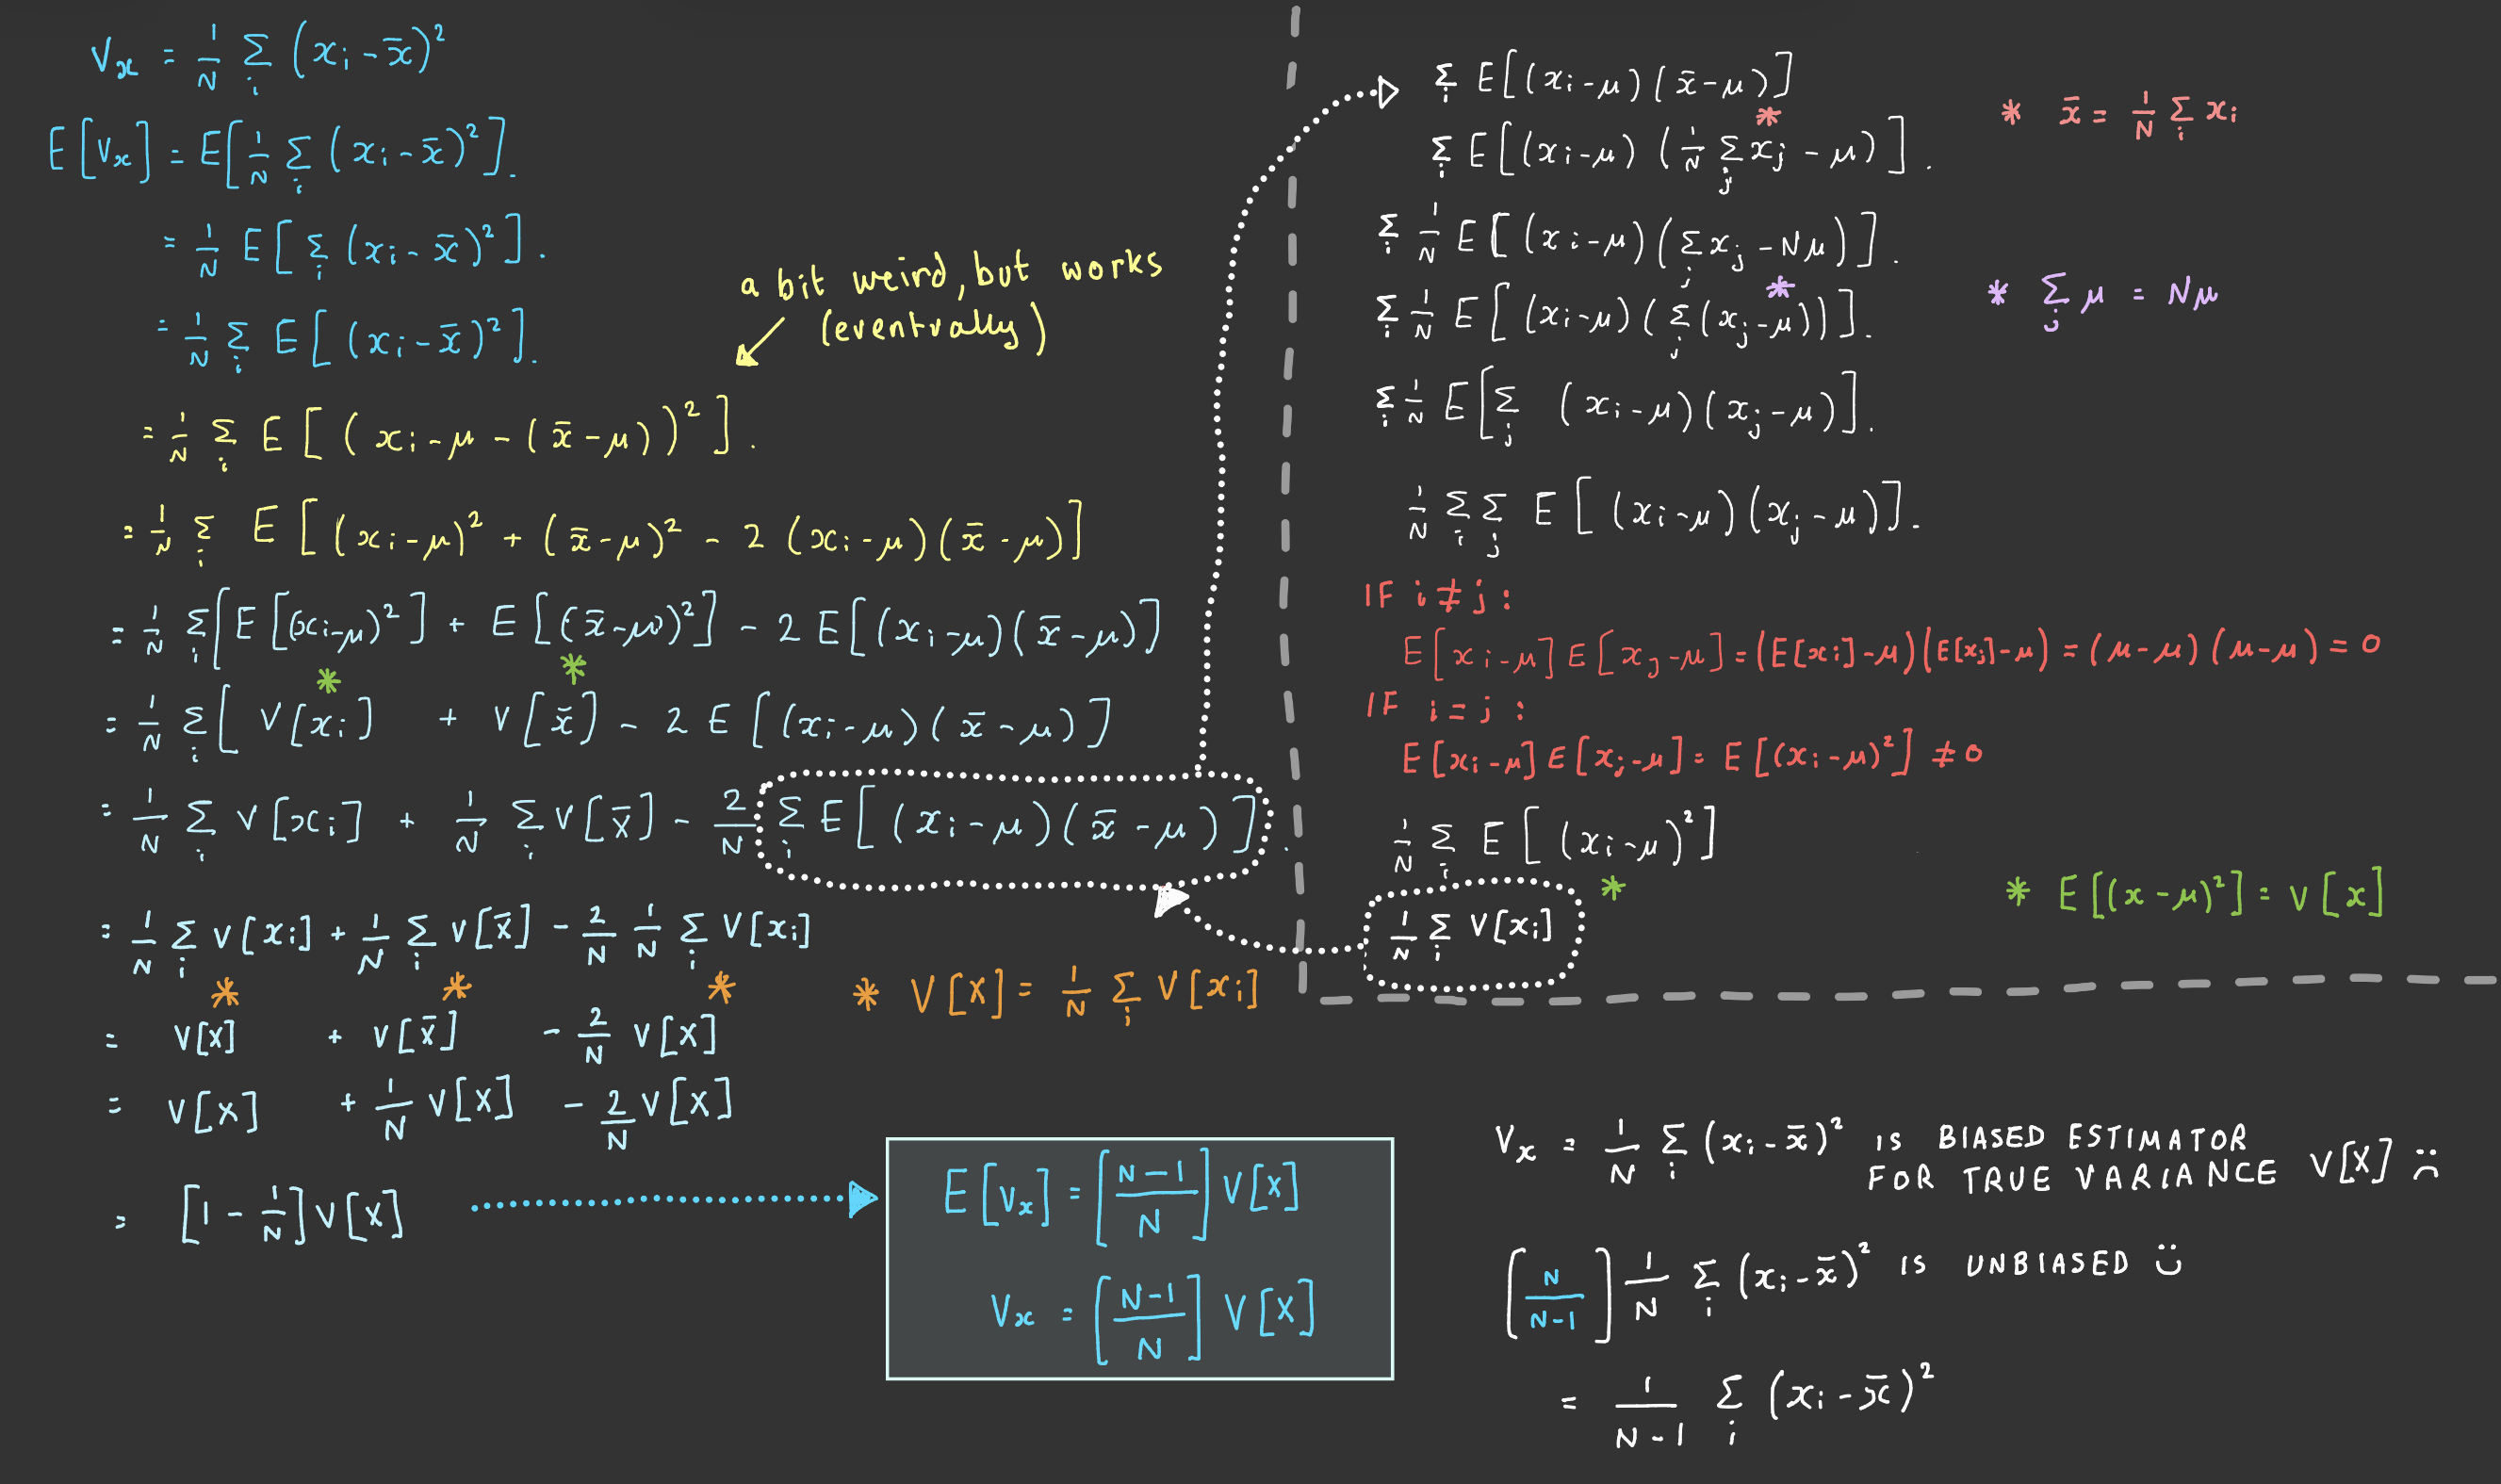
\includegraphics[scale=0.23]{var-proof-long.png}
\end{frame} 


% SAMPLE VARIANCE AS ESTIMATOR FOR TRUE VARIANCE
\begin{frame}{Sample Variance: Estimator \rbl{ \only<1>{Consistency}\only<2>{Bias} 
}
}
\footnotesize
%The Sample Variance: $\bbl{V[x_{_{N}}] }= \magtn{ \dfrac{1}{N} \sum\limits_i^N (x_i-\overline{x})^2}$ is an \bbl{Estimate, $\hat{V}[X]$} for the true variance $V[X]$.  \\[1ex]
We have shown that: \bhl{$\hat{V}[X]  = V[x_{_{N}}] = \dfrac{N-1}{N} V[X] $}\\[2ex]

\only<1>{
\boo{Consistency Check}: Does $\hat{V}[X] \rightarrow V[X]\; as \; N\rightarrow \infty$?\\[1ex]

%In this case the check is: $V[x_{_{N}}]  \rightarrow V[X]\; as \; N\rightarrow \infty$\\[1ex]

We can see that in the Asymptotic Limit ($N\to\infty$), $ \dfrac{N-1}{N} \to 1$ \\[2ex]

\ghl{The Sample Variance is a Consistent Estimator for the True Variance.}\;\;\tick
}

\only<2>{
\boo{Bias Check}: $b = E[\hat{V}[X]] - V[X]$\\[1ex]

%In this case the check is: $b = E[ V[x] ] - V[X] $\\[1ex]
%$E\left[\dfrac{N-1}{N} V[X]  \right] = \dfrac{N-1}{N} V[X] $, so $E[V[x_{_{N}}] ] = V[x_{_{N}}] $


The bias is $b = \dfrac{N-1}{N} V[X]  - V[X]  =  \dfrac{N-1-N}{N} V[X]  =  - \dfrac{1}{N} V[X]   $\\[1ex]

\yhl{The Sample Variance is a Biased Estimator for the True Variance.}\;\;\nope\\[1ex]

We could use the Unbiased Sample Variance, $V[x_{_{N-1}}] = \dfrac{1}{N-1} \sum\limits_i^N (x_i - \overline{x})^2$, \bbl{but bias is not the only factor in deciding which estimator is best...more next week}.
}
\end{frame} 

\begin{frame}{The Sample Variance is a Biased Estimator}
\footnotesize
Does it make sense that the Sample Variance $V[x_{_{N}}] = \dfrac{1}{N} \sum\limits_i^N (x_i-\overline{x})^2$ is biased?\\[1ex]

 \magtn{$b = E[\hat{\theta}]-\theta =  \rbl{-} \dfrac{1}{N} \theta$}: the bias is \rbl{negative}, because $E[\hat{\theta}]$ is \rbl{smaller} than the true variance $\theta$.\magt{*}\\[1ex]
 
 We can make sense of this if we consider the data used in each case. \bbl{The Sample Variance uses a limited number of measurements, $N$. These measurements determine the sample mean, $\overline{x}$, and are therefore clustered around the sample mean.}\\[1ex]
 
The value of the True Mean is formed by all possible measurements, so it makes sense that the true variance will be larger than the sample variance. The larger $N$ gets, the closer we get to `all possible measurements', so the bias reduces.\\[1ex] 

\notsotiny
\magt{*Using $E[\hat{\theta}] \equiv E[\hat{V}[X]] \equiv E[ V[x_{_{N}}] ]$ and $\theta \equiv V[X]$ for neatness.}

\end{frame}

%\begin{frame}{Minimum Variance Bound}
%\footnotesize
%We skipped the variance of the sample mean and sample variance in the interests of time, but you can find them in books or on the internet. I recommend using more than one source.\\[1ex]
%
%The (Rao-Cramer-Frechet) RCF Inequality, also known as the \boo{Information Inequality}, provides a \boo{Minimum Bound} on the variance of an estimator:\\[1ex]
%
%$V[\hat{\theta}] \geq 
%\left\{ N E\left[
%\left(
%\dfrac{ \partial \ln f_Y(y;\theta) } { \partial \theta } 
%\right)^2
%\right]
% \right\}^{-1}
% =
% \left\{ - N E\left[
%\left(
%\dfrac{ \partial^2 \ln f_Y(y;\theta) } { \partial \theta^2 } 
%\right)
%\right]
% \right\}^{-1}
% =
% \mathcal{I}^{-1}(\theta)
% $
%
%\magt{$\dfrac{d \ln \theta }{d\theta} = \dfrac{1}{\theta} $}\\[1ex] 
%
%$\mathcal{I}(\theta)$ is known as the \boo{Fisher Information}.
%
%\end{frame}

%. LIKELIHOOD!!!

\section{Likelihood \& Bayes}

\begin{frame}{A Reminder of the Likelihood }
\footnotesize
\only<1>{
When we calculate probabilities, we assume a known parameter, eg $\lambda$ or $p$. The general symbol for any such parameter, or set of them, is $\theta$.\\

Sometimes we may not know the parameter value, and wish to Estimate it based on the distribution of our \magtn{data}. We can do this by trying out a bunch of different parameter values and seeing which gives us the `closest match' in shape to the distribution of our \magtn{data}. The parameter that results in the closest match is the one with the highest Likelihood, $\mathcal{L}_{\theta}$.\\

The Likelihood $\mathcal{L}_{\theta}$ of a parameter value $\theta$ being the correct one, \magt{given the data}, is:
\begin{center}
\bhl{$\mathcal{L}_{\theta}= \magtn{\prod\limits_i^N}\, f_Y(\magtn{y_i}; \theta) $}\\[3ex]
\end{center}

}

\only<2>{
\begin{center}
\bhl{$\mathcal{L}_{\theta}= \magtn{\prod\limits_i^N}\, f_Y(\magtn{y_i}; \theta) $}\\[3ex]
\end{center}
The Likelihood is the product of the PDF $f_Y$ \magtn{evaluated at each data measurement $y_i$}. The \magtn{product is over the $N$ data measurements}. $\theta$ is the parameter value (or set of) that we are trying out. The parameter value that best describes the data is the one with the highest $\mathcal{L}_{\theta}$. We recalculate $\mathcal{L}_{\theta}$ for each value of $\theta$ we want to try out using the above formula.\\[1ex]

\boo{Wait, didn't you say that the PDF evaluated at a given value is zero?! }\\[1ex]

Yes I did! The difference here is that each data measurement represents a range of values, rather than a single value (we can't define a single value from a continuous set of real numbers). Measurements are always discrete, even when the RV we are measuring is continuous. So, $f_Y(y_i;\theta)\neq 0$.\\
}
\only<3>{
In preparing these slides I went back to the week 3 Functions lecture to steal some \LaTeX{}, and \rbl{found an error}\magt{*} in my definition of the Likelihood. Sorry!\\[1ex]

This is an important definition that I wrote down completely backwards.\magt{*}\\
The Normalised Likelihood is the Probability of $\theta$, given the data.\; \nope\\[1ex]

I have corrected this on the slides: \\
\ghl{The Normalised Likelihood is the Probability of the \bf{data, given $\theta$}.}\;\;\tick\\[1ex]

Let's go back to Bayes-ics (sorry) to check we understand.\\[1ex]

\magt{*A frequentist would say that what I wrote was not in error, because the two statements mean the same thing. But this is not the case for the Bayesian approach, which is what I was attempting to convey. So it was an error. }

}


\end{frame} 


\begin{frame}{A Reminder of Bayes' Theorem}
\small
\only<1>{
\begin{center}
$P(A | B) = \dfrac{ P(B|A)P(A) }{ P(B) }$\\[3ex]
\end{center}
All of the Ps in here are \gbl{valid} PDFs (or PMFs): they have integral (or sum) equal to 1.\tick \\[1ex]
}

\only<2->{
Let A $\rightarrow \theta$: the parameter values, and B $\rightarrow y$: the data.\\[1ex]
}


\only<2>{
\begin{center}
$P(A | B) = \dfrac{ P(B|A)P(A) }{ P(B) }$ \;\;\; \Large{\ding{234} }\normalsize\;\;\;\bhl{$P(\theta | y) = \dfrac{ P(y|\theta)P(\theta) }{ P(y) } $}\\[3ex]
%\ding{220}  \ding{224}  \ding{225}  \ding{234}  \ding{229} 
\end{center}
Are all of the Ps still \gbl{valid}?\\[1ex]
}

\only<3>{
\begin{center}
$P(\theta | y) = \dfrac{ P(y|\theta)\bbl{P(\theta)} }{ P(y) } $\\[3ex]
\end{center}
\bbl{$P(\theta)$ is the Total Probability that the correct value of our parameter is ... anything!} \tick\\
}
\only<4>{
\begin{center}
$P(\theta | y) = \dfrac{ P(y|\theta)P(\theta) }{ \bbl{P(y)} } $\\[2ex]
\end{center}
\bbl{$P(y)$ is the Total Probability of our data having any value.} \tick\\ 
}

\only<5>{
\begin{center}
$P(\theta | y) = \dfrac{ \bbl{P(y|\theta)}P(\theta) }{ P(y) } $\\[2ex]
\end{center}
\bbl{$P(y|\theta)$ is the probability of observing all the data, given any parameter value is correct.} \tick\\ 
}

\only<6>{
\begin{center}
$\bbl{P(\theta | y)} = \dfrac{ P(y|\theta)P(\theta) }{ P(y) } $\\[2ex]
\end{center}
\bbl{$P(\theta|y)$ is the probability of any parameter value being correct, given all the data.}\tick\\ 
}

\end{frame}


\begin{frame}{A Reminder of Bayes' }
\small

\only<1-3>{
The next step is to consider how we can use this to talk about the probability of a specific parameter $\theta_i$ being the correct one. \\[3ex]
}
\only<1>{
\begin{center}
$P(\theta | y) = \dfrac{ P(y|\theta)P(\theta) }{ P(y) } $\\[3ex]
\end{center}
Let's see what happens...\\
}
\only<2>{
\begin{center}
$P(\rbl{\theta_i} | y) = \dfrac{ P(y|\rbl{\theta_i})P(\rbl{\theta_i}) }{ P(y) } $\\[3ex]
\end{center}
\boo{We have broken Bayes!} The Ps are no longer (necessarily) valid! They have some meaning, but they are not (necessarily) Probabilities.\\[1ex]
}
\only<3>{
\begin{center}
$P(\rbl{\theta_i} | y) = \dfrac{ P(y|\rbl{\theta_i})P(\rbl{\theta_i}) }{ \bbl{P(y)} } $\\[3ex]
\end{center}
%\boo{We have broken Bayes!} The Ps are no longer valid! They have some meaning, but they are not Probabilities.\\[1ex]
We must fix this! Let's work with our one remaining valid P, \bbl{$P(y)$}. \\[1ex]
}


\only<4>{
\bbl{$P(y) =\int P(y,\theta)\, d\theta $} is a Marginal P of the Joint P $P(y,\theta)$.\\[2ex]
\magtn{Recall $f_Y(y) = \int\limits_{-\infty}^{\infty} f_{YZ}(y,z) dz$} - we `integrate out' the other RV.\\[2ex]

\begin{center}
$P(\theta_i | y) = \dfrac{ P(y | \theta_i)P(\theta_i) }{ \bbl{\int P(y,\theta)\, d\theta} } $\\[3ex]
\end{center}
}
\only<5>{
\bbl{$P(y,\theta) = P(y|\theta)\,P(\theta)$: the Joint P can be written as the Conditional P times the Marginal P.} \\[2ex]
\magtn{Recall $P(A\cap B) = P(A|B)P(B)$}.\\[2ex]
\begin{center}
$P(\theta_i | y) = \dfrac{ P(y | \theta_i)P(\theta_i) }{ \bbl{\int P(y|\theta)P(\theta) d\theta} }$\\[3ex]
\end{center}
}

\only<6>{
With the new expression in the denominator \bbl{$P(y) =\int P(y | \theta) P(\theta) d\theta$} we can clearly show that \gbl{the LHS} \textbf{is} a valid probability: \\[5ex]
$\int \gbl{ P(\theta_i | y)} d\theta
= \displaystyle \int  \dfrac{ 
P(y|\theta_i)
P(\theta_i) 
}{
 \bbl{\int P(y | \theta_i) P(\theta_i) d\theta}
 }d\theta
=  \dfrac{ \int 
P(y|\theta_i)
P(\theta_i) d\theta
}{
 \bbl{\int P(y | \theta_i) P(\theta_i) d\theta}
 }=1
 $\\[2ex]
 
 This is important, because it means that the Posterior probability $\gbl{ P(\theta_i | y)}$ for a specific parameter $\theta_i$, given the data, is a valid PDF.
}
\end{frame}


\begin{frame}{A Reminder of Bayes' }
\small
\only<1>{
\gbl{$P(\theta_i | y)$}, the Posterior probability distribution for the correct parameter being $\theta_i$, given the data $y$, is a valid PDF. \tick \\[3ex]
\rbl{The so-called Ps on the RHS are not (necessarily) valid PDFs.}\\[1ex]

\begin{center}
$P(\theta_i | y)  =  \dfrac{ P(y|\theta_i) P(\theta_i) }
{ \int P(y | \theta_i) P(\theta_i) d\theta }$\\[2ex]
\end{center}

Let's fix this, sharpish.
}

\only<2>{
\rbl{$P(\theta_i)$ is the Prior} of the specific parameter $\theta_i$ being the correct one. We gave the Prior a special symbol $\pi(\theta_i)$ - we are going to get confused if we keep the P there, because it is not necessarily a valid PDF. \nope\\[1ex]

\begin{center}
$\gbl{ P(\theta_i | y)}  =  \dfrac{ P(y|\theta_i) \rbl{P(\theta_i)} }
{ \int P(y | \theta_i) \rbl{P(\theta_i)} d\theta }$\\[2ex]
\end{center}
}

\only<3>{
\gbl{$\pi(\theta_i)$ is the Prior} of the specific parameter $\theta_i$ being the correct one. We gave the Prior a special symbol \gbl{$\pi(\theta_i)$} because it is not necessarily a valid PDF. \gbl{That's better}.\\[1ex]

\begin{center}
$P(\theta_i | y)  =  \dfrac{ P(y|\theta_i) \gbl{\pi(\theta_i)} }
{ \int P(y | \theta_i) \gbl{\pi(\theta_i)} d\theta }$\\[2ex]
\end{center}
}

\only<4>{
\rbl{$P(y | \theta_i)$ is the Likelihood} of observing the data given that a specific parameter $\theta_i$ is the correct one. We gave this Likelihood a special symbol \rbl{$\mathcal{L}_{\hat{\theta}}$}. On its own, it is not necessarily a valid PDF.\nope\\[1ex]

\begin{center}
$P(\theta_i | y)  =  \dfrac
{ \rbl{P(y|\theta_i)} \gbl{\pi(\theta_i)} }
{ \int \rbl{P(y | \theta_i)} \gbl{\pi(\theta_i)} d\theta }$\\[2ex]
\end{center}
}

\only<5>{
\gbl{ $\mathcal{L}_{\theta}$  is the Likelihood} of observing the data given that a specific parameter $\theta_i$ is the correct one. On its own, it is not a valid PDF. \gbl{That's better.}\\[1ex]

\begin{center}
$P(\theta_i | y)  =  \dfrac
{\gbl{\mathcal{L}_{\theta}} \gbl{\pi(\theta_i)} }
{ \int \gbl{\mathcal{L}_{\theta}} \gbl{\pi(\theta_i)} d\theta }$\\[2ex]
\end{center}
}

\only<6>{
Now we are happy. \tick \tick \tick \tick \tick \tick \tick \tick \tick \\[3ex]

\begin{center}
\ghl{
$P(\theta_i | y)  =  \dfrac
{ \mathcal{L}_{\theta}\, \pi(\theta_i) }
{ \int \mathcal{L}_{\theta}\, \pi(\theta_i)\, d\theta }$
} \\[2ex]
\end{center}

Later on we will see that the denominator is just a normalising factor, and the Posterior is $\propto \mathcal{L}_{\theta} \times \pi(\theta)$. For the Frequentist, the Posterior is just the (normalised) Likelihood.  
}

\end{frame}




%\only<1>{
%Recall Bayes Theorem: \hspace{1cm} Bayesian  \hspace{2cm}  \textcolor{purr}{Frequentist}\\[1ex]
%$P(H_i | X) = \dfrac{ P(X|H_i) \pi(H_i) } {  \sum\limits_i^N P(X | H_i) \pi(H_i) } \rightarrow \dfrac{ P(x|\theta) \pi(\theta) } {  \int P(x | \theta) \pi(\theta) d\theta }  \rightarrow \textcolor{purr}{\dfrac{ P(x|\theta)  } {  \int P(x | \theta)  d\theta } } = P(\theta|x)$
%}


\section{Intro to MLE \& LSE}




\begin{frame}{The Maximum Likelihood: Intro}
\footnotesize

$\mathcal{L}_{\theta}$ is the Likelihood of observing the data given that a specific parameter $\theta_i$ is the correct one.\\[1ex]

The value $\theta_i$ that \boo{Maximises the Likelihood} is, by definition, the best Estimate $\hat{\theta}$ for the true parameter $\theta$.\\[1ex]

\begin{center}
\bhl{$\mathcal{L}_{\theta}= \prod\limits_i^N\, f_Y(y_i; \theta) $}\\[3ex]
\end{center}

To find the maximum of a function, we differentiate it, and set the result to zero. This is because \boo{the first derivative of a function at a given point is its Gradient}.
\end{frame} 

\begin{frame}{The Maximum Likelihood}
\footnotesize

\begin{center}
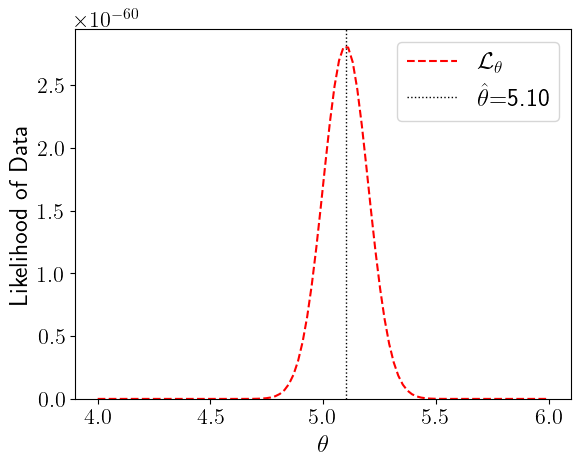
\includegraphics[scale=0.55]{PLOTDAT6-LikevMU.png}
\end{center}

%To find the maximum of a function, we differentiate it, and set the result to zero. This is because \boo{the first derivative of a function at a given point is the Gradient}.
\end{frame} 



\begin{frame}{The Maximum Likelihood Estimator (MLE)}
\footnotesize
%$\mathcal{L}_{\theta}$ is the Likelihood of observing the data given that a specific parameter $\theta_i$ is the correct one.\\
The value $\theta_i$ that \boo{Maximises the Likelihood} is, by definition, the best Estimate $\hat{\theta}$ for the true parameter $\theta$.\\
\begin{center}
\bhl{$\mathcal{L}_{\theta}= \prod\limits_i^N\, f_Y(y_i; \theta) $}\\[3ex]
\end{center}
\begin{itemize}
\item We can use the MLE when we know the form of the PDF ($f_Y$) but not its parameter values. 
\item The MLE method works by evaluating $\mathcal{L}_{\theta}$ for different $\theta_i$ to determine the value that maximises $\mathcal{L}_{\theta}$.
\item We shall see later on that maximising the Likelihood is equivalent to \boo{Minimising The Residuals}.
\end{itemize}
\end{frame} 


\begin{frame}{Residuals}
\footnotesize
\begin{itemize}
\item A dataset $y = \{y_i, ..., y_N \}$ contains the measured values of a RV $Y$ from some underlying PDF $f_Y(y;\theta)$.
\item \magtn{The Residual} for the $i^{th}$ measurement is \bhl{$y_i - \mu$}: a measure of how far the measurement $y_i$ deviates from the True Mean $\mu\equiv E[Y]$.
\item The \magtn{Standardised Residual} for the $i^{th}$ measurement is \bhl{$\dfrac{y_i - \mu}{\sigma_i} = \dfrac{y_i - \mu}{y_i - \overline{y}}$}.
\end{itemize}
\vspace{0.5cm}

To calculate the \magtn{Residual}, $y_i - \mu$, we must know (or estimate) the underlying distribution for our data, as $\mu$ is not (necessarily) a statistic of the data but a parameter of the true distribution. However, if we estimate $\mu$ from the data, then the residual is a statistic of the data.\\[1ex]

The denominator is the \magtn{Measurement Uncertainty} $\sigma_i = y_i - \overline{y}$. This is a statistic, purely data-based, making no assumptions as to the underlying distribution.\\[1ex]


\end{frame} 


\begin{frame}{Chi Squared}
\footnotesize
\boo{Pearson's Chi Squared, $\chi^2$,} is  the sum of the squared standardised residuals:\\
\begin{center}
\bhl{$\chi^2 = \sum\limits_i^N \dfrac{ (y_i - \mu)^2}{V[y_i]} $} \\[1ex]
\end{center}

\bbl{We will become familiar with this. For now, notice that the smaller $\chi^2$ is, the closer (on average) our measurements are to the expectation.}\\[1ex]

\magt{Out in the world} you will see the standardised residual written as \magtn{$\frac{obs\;-\;exp}{\sqrt{exp}}$}, where obs and exp are  counts (numbers).  We will see later that this is the form used for Binned Data (histograms), because in that case we estimate the statistical uncertainty on the number of entries in a given bin as $\sigma_{bi} = \sqrt{N}$, where $N$ is the number of expected entries in the bin. This is known as Poisson statistics, or `counting statistics'.

\end{frame} 



\begin{frame}{Least Squares}
\footnotesize
\only<1>{
\begin{center}
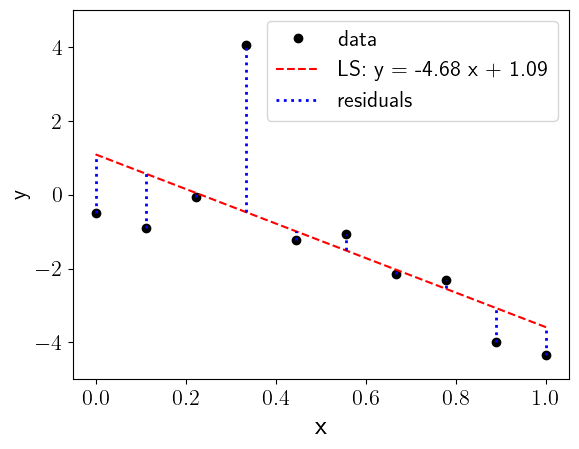
\includegraphics[scale=0.6]{LinearLeastSquaresExample_c1.0_m-5.2_noise2.4_outliers2.png}
\end{center}
}

\only<2>{
\begin{multicols}{2}
When I hear the term Least Squares I think of sitting in an undergrad laboratory trying to fit a line to some data points such that the deviations between the data points and the line are as small as possible. \\

This means \boo{Minimising The Residuals}.\\[1ex]

I think one reason why Least Squares is used so prolifically is that it is understandable visually. Do not underestimate the power of a good plot.

\begin{center}
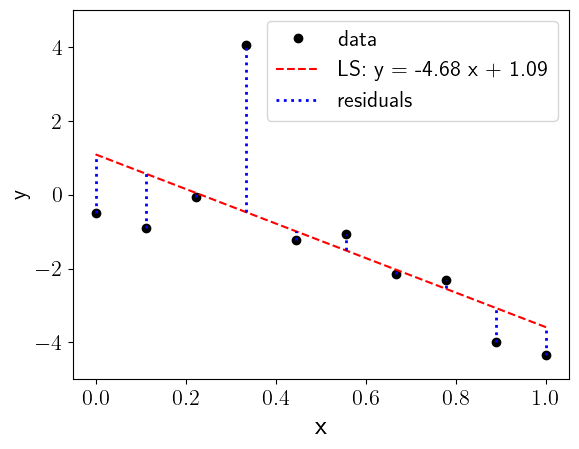
\includegraphics[scale=0.36]{LinearLeastSquaresExample_c1.0_m-5.2_noise2.4_outliers2.png}
\end{center}
\end{multicols}
}
\only<3>{
\begin{multicols}{2}
%For those who haven't been blessed with such experiences,
The method is called Least Squares because it chooses the (best fit) line for which the sum of the squared residuals (Squares) is minimised (Least).\\[1ex]

We can fit any line or curve (any functional form) to data points - we don't need to know what the functional form is in advance, because we can try everything! It does help to have an educated guess to start with, though.\\[1ex]% which is why it is imperative to look at (plot!) the data before trying to fit it. \\[1ex]
\begin{center}
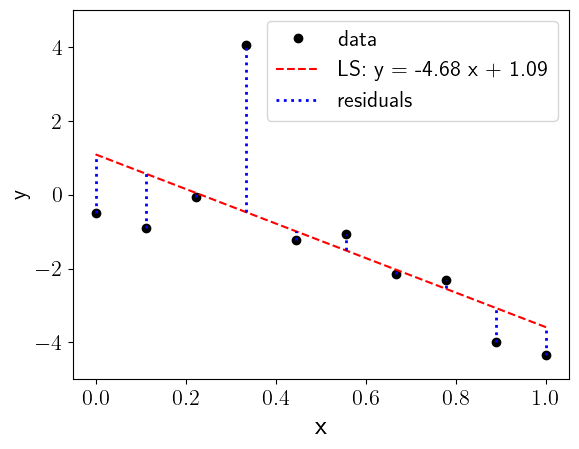
\includegraphics[scale=0.35]{LinearLeastSquaresExample_c1.0_m-5.2_noise2.4_outliers2.png}
\end{center}
\end{multicols}
}
\end{frame} 



\begin{frame}{LSE and MLE: Point Estimators for Parameters}
\footnotesize
Both Least Squares and Max Likelihood are Point Estimators for finding the parameter Estimates that Maximise  $\mathcal{L}_{\theta}$ by Minimising the Residuals.\\
\begin{itemize}
\item Least Squares looks pretty easy and intuitive, and we can see the residuals directly, but it's not yet clear how they relate to the Likelihood...
\item Maximising the Likelihood just looks like math, and although I said it is related to minimising the residuals, I have not yet given you any idea of how (other than a slide last week where I showed the log of a Normal PDF...)
\end{itemize}

\bbl{To use LSE} we need to have a really good grasp of our uncertainties (error bars) because the larger the error bars, the more possibilities there are for curves that will fit the data. We can do basic LSE with just a few data points, hence its popularity in undergraduate labs.\\[1ex]

\bbl{To use MLE} we need to know the underlying PDF, and we need a pretty good amount of data for MLE to work its magic.\\[1ex]

\end{frame}


\begin{frame}{The Log Likelihood}
\footnotesize
Logarithms are very handy. Recall \ghl{$\ln{(abc)} = \ln{a} + \ln{b} +\ln{c}$}\\[1ex]

%Also recall the Likelihood is a product of PDFs: $\mathcal{L} = \prod\limits_i^N f_X (x_i;\theta_i)$\\[1ex]

\bbl{The Log of a product is the sum of logs:}\\

\begin{center}
\bhl{$\ln{ \mathcal{L} } = \ln{\left( \prod\limits_i^N f_X (x_i;\theta_i)\right)} =  \sum\limits_i^N \ln{ f_X (x_i;\theta) }$}\\[2ex]
\end{center}

The sum is over the PDF evaluated at each of the $N$ data measurements $x_i$.\\[1ex]

It is generally much easier to work with the log likelihood than the likelihood.\\[1ex]

%Recall: $\mathcal{L}_{\hat{\theta}}$ is the Likelihood of observing the data given that a specific parameter $\hat{\theta}=\theta_i$ is the correct one\\[1ex]
\end{frame}

\begin{frame}{The Negative Log Likelihood}
\footnotesize
The  Log Likelihood $\ln{ \mathcal{L} } =  \sum\limits_i^N \ln{ f_X (x_i;\theta) }$  is always negative, because $\ln{(a)}<0 $ for $a<1$, and $f_X(x_i;\theta)$ must always be less than 1.\\[1ex]

Because the Log Likelihood is negative and \magtn{we like positive numbers*}, we pop a minus sign on the front and use the Negative Log Likelihood for our calculations.\\[1ex]

\begin{center}
\bhl{$ - \ln{\mathcal{L}} = - \sum\limits_i^N \ln  f_X(x_i;\theta)$}\\[1ex]
\end{center}

Maximising the Likelihood is equivalent to Minimising the Negative Log Likelihood.\\[1ex]

\magtn{*This is me being silly. Finding the Point Estimate $\hat{\theta}$ is easiest using \texttt{scipy.optimize} methods, and optimisers are minimisers rather than maximisers, by convention.}

\end{frame}


\begin{frame}{Likelihood, Log Likelihood, and Negative Log Likelihood}
\footnotesize
\only<1>{ \bbl{Likelihood $\mathcal{L}_{\theta}$}: Maximum at $\hat{\theta}$\\[1ex] }
\only<2>{ \bbl{Log Likelihood $\ln \mathcal{L}_{\theta}$}: Maximum at $\hat{\theta}$ and we can see the tails!\\[1ex]}
\only<3>{ \bbl{Negative Log Likelihood $- \ln \mathcal{L}_{\theta}$}: Minimum at $\hat{\theta}$ and we can see the tails!\\[1ex]}

\only<1>{\begin{center} 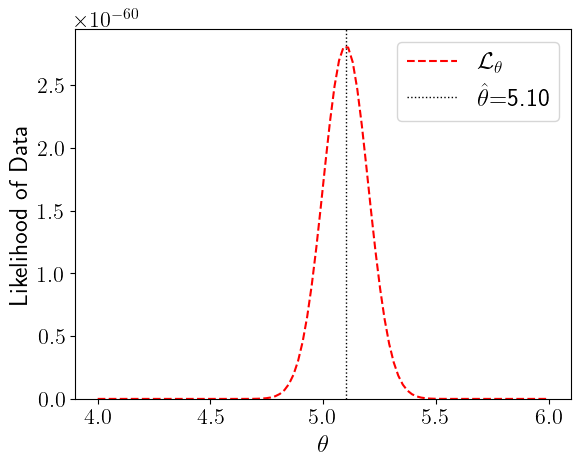
\includegraphics[scale=0.35]{PLOTDAT6-LikevMU.png} \end{center}}
\only<2>{\begin{center} 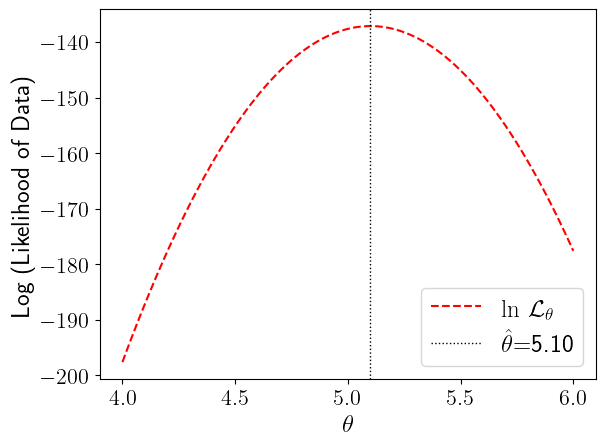
\includegraphics[scale=0.35]{PLOTDAT6-LogLikevMU.png} \end{center}}
\only<3>{\begin{center} 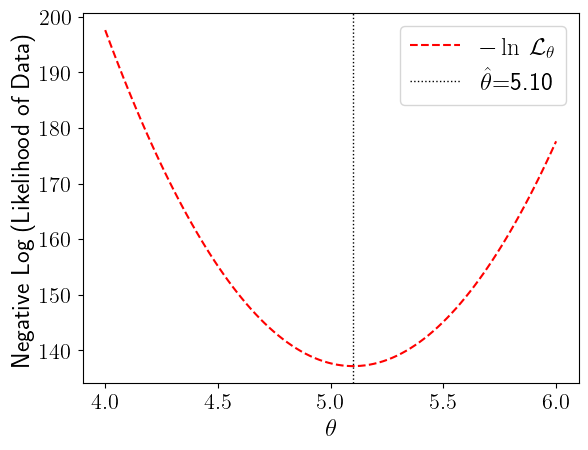
\includegraphics[scale=0.35]{PLOTDAT6-NegLogLikevMU.png} \end{center}
\magtn{All the same information that was in the Likelihood $\mathcal{L}_{\theta}$ is in the Negative Log Likelihood $-\ln \mathcal{L}_{\theta}$, it is just nicer to work with $- \ln \mathcal{L}_{\theta}$.}
}






\end{frame}





\begin{frame}{Thanks For Your Time}
\center
\Huge
Fin.
\end{frame}






\end{document}
